\documentclass[10pt, onecolumn]{IEEEtran}

\usepackage{etoolbox}
\usepackage{scrextend}
\usepackage{graphicx}

% remove \centering from \section
\patchcmd{\section}{\centering}{}{}{}

\begin{document}
\title{An Analysis of Risk\\ in Open-Source Projects}

\author{\IEEEauthorblockN{Róisín Ní Bhriain}
\IEEEauthorblockA{\\Student Number: 23269640\\}
\and
\IEEEauthorblockA{Sneha Dechamma Mallengada Suresh\\
    Student Number: 23262168\\}}

\maketitle

\begin{description}
    \item[]
    \begin{center}
        \item[\textbf{Technical Manual - 23-07-2024}] 
        \end{center}
    \item[]
\end{description}



\begin{abstract}
\begin{addmargin}[4em]{4em}
This paper explores the methods used in the prediction of risk when using open-source software. There are a number of methods used and the aim is to combine these to give a more comprehensive view of the risks in using a particular open-source project. We examine the literature to decide on an appropriate prediction algorithm for each section. We provide a graph of the final results which can be used to aid in finding where the risk lies in the dependency trees. 
\end{addmargin}
\end{abstract}


\section{Introduction}
In November 2021 a vulnerability was discovered in the popular open-source logging library Apache Log4j. This software is widely used in web portals. The vulnerability in this package means that hackers can run malicious code remotely on a victim's machine (H. Gupta, A. Chaudhary, and A. Kumar, 2022). The main aim of the log4j vulnerability is to obtain Lightweight Directory Access Protocol information and this will serve as a gateway to full control of the machine. The attack works with several steps: information gathering, weaponisation, delivery, exploitation and installation (F. Maulana et al., 2023). 

This paper explores the prediction of risks in maven dependency trees through examining both GitHub project activity and NVD vulnerability CVEs. ARIMA prediction is used for both sets of data based on user configuration data and returns a coloured graph based on the analysed risk. 

\section{Related Work}

\subsection{Project Metadata Analysis}


\subsection{Vulnerability CVE Data Analysis}

\section{Methodology}
This section explores the prediction of risk methods that we used.

\subsection{Finding Dependencies Algorithm}
To find dependencies of different projects we focused on Maven dependency trees. We first extract each of the 

\subsection{Project Meta-Data Prediction}

\subsection{Vulnerability Database Prediction}

\subsection{Risk Calculations}
In terms of calculating risk we implemented some configurations options for a user to decide how many commits, days-to-close issues, and vulnerabilities per month are acceptable. 


\[( x / numDaysToFixIssues ) * 10\]

\[( numCommits / x ) * 10\]

\[( x / vulsCountPerMonth ) * 10\]

These are the calculations we used for the risk scores for each of the sections. There is the option to decide project activity based on issues fix time, commits per month or both. The user supplies the configuration options of \textit{numDaysToFixIssues}, \textit{numCommits}, and \textit{vulCountsPerMonth}. That way the acceptable levels of risk are set. The idea is that they are then assigned a risk score: where not enough is < 0, 0-2.5 is low risk, 2.5-5 is medium risk, 5-7.5 is high risk and > 7.5 is severe risk. 

\begin{figure}
    \centering
    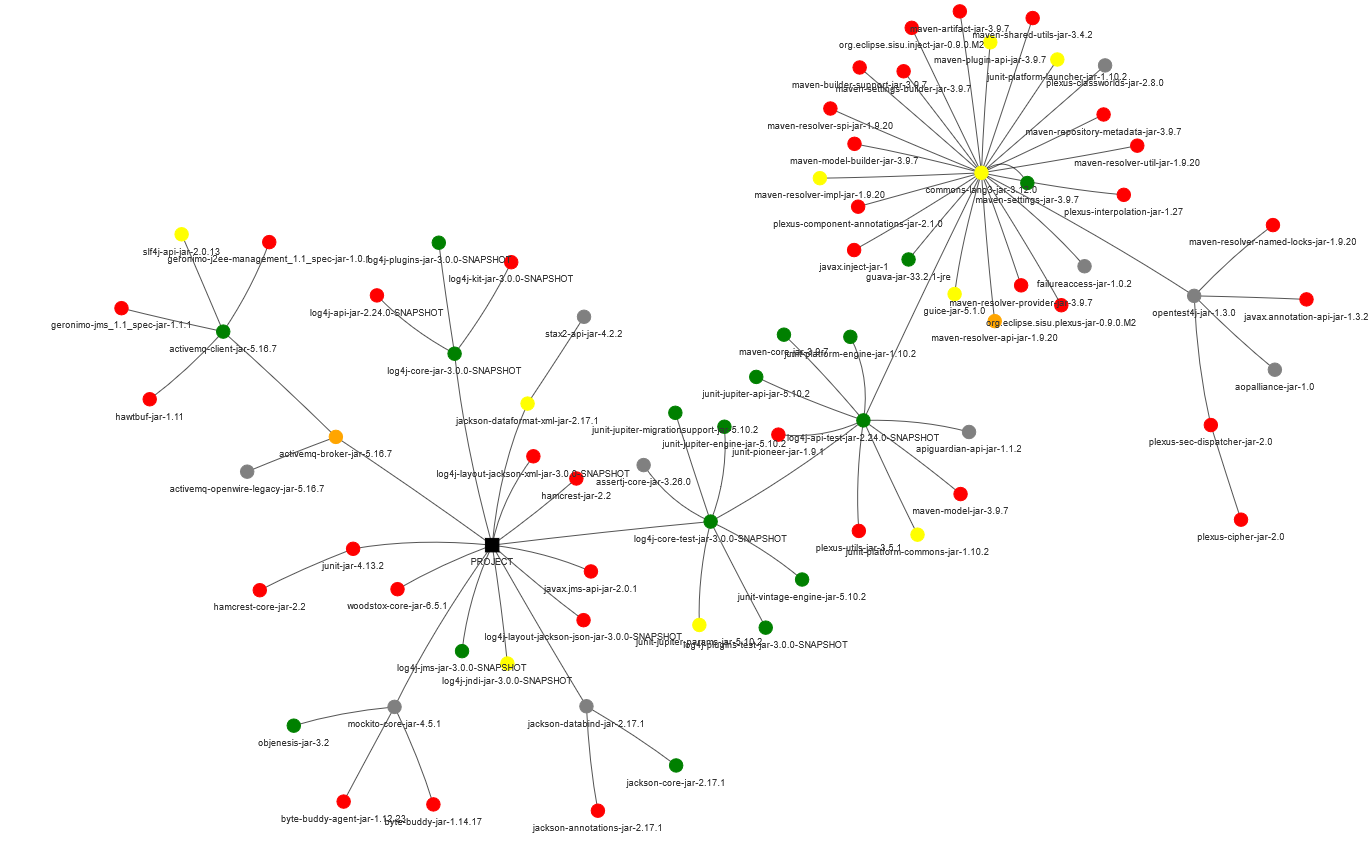
\includegraphics[width=01\linewidth]{image.png}
    \caption{Dependency Tree With Risk Levels Colour Coded} 
\end{figure}

Fig 1 shows a final dependency tree with colour coded risk evaluations of each of the dependencies.


\section{Results \& Evaluation}
For the evaluation of the predictions in this project we used the commonly used metrics: Mean absolute percentage error (MAPE), mean absolute error (MAE), and root mean squared error (RMSE). 

\section{Conclusions \& Further Work}
For the purpose of this practicum we focused on examining maven dependency trees which is primarily used for Java projects. Further work could be done to examine other package manager dependency trees such as \textit{PyPI} for Python, \textit{NPM} for JavaScript, and \textit{Conan} for C. 

\begin{thebibliography}{1}

\bibitem{IEEEhowto:kopka}
H.~Kopka and P.~W. Daly, \emph{A Guide to \LaTeX}, 3rd~ed.\hskip 1em plus
  0.5em minus 0.4em\relax Harlow, England: Addison-Wesley, 1999.

\end{thebibliography}

\appendices
\section{Graphs}
This section contains other important graphs that we did not include in the main body of the project.


\ifCLASSOPTIONcaptionsoff
  \newpage
\fi

\end{document}


